\begin{examplebox}
\textbf{\textcolor{CExample}{例1｜两个不同根都在区间内（基础）}}\par
\textbf{题目：}$f(x)=x^2+2x+t$在$(-2,1)$内有两个不同零点，求$t$。
\par\textbf{第一步：}有两根，$\Delta=4-4t>0\Rightarrow t<1$。
\par\textbf{第二步：}对称轴$x_0=-1$，满足$-2<-1<1$。
\par\textbf{第三步：}$a=1>0$，两端均要在轴上方：$f(-2)=t>0$，$f(1)=t+3>0$，合起来$t>0$。
\par\textbf{答案：}\boxed{0<t<1}。例如取$t=\frac12$，两根$-1\pm\frac{\sqrt2}{2}$，确实都在$(-2,1)$内。
\begin{center}
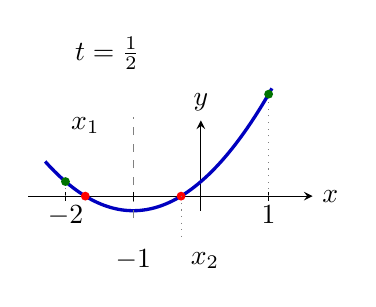
\begin{tikzpicture}[x=.86cm,y=.37cm,>=stealth]
 \draw[->] (-2.55,0)--(1.65,0) node[right]{$x$};\draw[->] (0,-.5)--(0,2.6) node[above]{$y$};
 \draw[very thick,blue!75!black,domain=-2.3:1.05,samples=75] plot (\x,{(\x+1)*(\x+1)-.5});
 \draw[dashed,gray] (-1,-.76)--(-1,2.7);
 \fill[red] (-1.7071,0) circle(1.6pt) (-.2929,0) circle(1.6pt);
 \node[below] at (-2,0) {$-2$};\node[below] at (-1,-1.5) {$-1$};\node[below] at (1,0) {$1$};
 \node[above] at (-1.7071,1.8) {$x_1$};\node[below right] at (-.2929,-1.6) {$x_2$};
 \foreach \v in {-2,-1,1}\draw (\v,.15)--(\v,-.15);
 \draw[dotted,gray] (-2,0)--(-2,.5) (1,0)--(1,3.5) (-.2929,0)--(-.2929,-1.4);
 \fill[green!45!black] (-2,.5) circle(1.6pt) (1,3.5) circle(1.6pt);
 \node[above right] at (-2,4.0) {$t=\frac12$};
\end{tikzpicture}

\end{center}

\medskip
\textbf{\textcolor{CExample}{例2｜一个零点，端点都不是根（进阶）}}\par
\textbf{题目：}$f(x)=x^2-2kx+4$在$(-1,1)$内恰一个零点，且$f(-1)f(1)\ne0$，求$k$。
\par\textbf{先考虑两端异号：}$f(-1)=5+2k$，$f(1)=5-2k$，
\[(5+2k)(5-2k)<0\iff k<-\tfrac52\ \text{或}\ k>\tfrac52.\]
\textbf{再排查重根：}$\Delta=4k^2-16=0\Rightarrow k=\pm2$，顶点$x_0=k$不在$(-1,1)$内，\textbf{因此没有遗漏的重根情形}。
\par\textbf{答案：}\boxed{k<-\frac52\ \text{或}\ k>\frac52}。
\begin{center}
\begin{tikzpicture}[x=1.28cm,y=.1122cm,>=stealth]
 \draw[->] (-1.4,0)--(1.38,0) node[right]{$x$};
 \draw[very thick,orange!80!black,domain=-1.12:1.17,samples=75] plot (\x,{\x*\x-6*\x+4});
 \draw[dotted,gray] (-1,0)--(-1,11) (1,0)--(1,-1);
 \fill[red] (.76393,0) circle(1.7pt);
 \node[below] at (-1,0) {$-1$};\node[below] at (1,-3) {$1$};\node[above right] at (.76393,.5) {$x_1$};
 \node[above] at (-.5,15) {$k=3$：异号，只穿一次};
\end{tikzpicture}

\end{center}

\medskip
\textbf{\textcolor{CExample}{例3｜一个零点，别漏掉端点根（综合）}}\par
\textbf{题目：}$f(x)=x^2+px+4$在$(1,3)$内恰有一个零点，求$p$（\textbf{题目没有排除端点为根}）。
\par\textbf{情况一：两端异号。}$f(1)=p+5$，$f(3)=3p+13$，
\[(p+5)(3p+13)<0\iff -5<p<-\tfrac{13}{3}.\]
\textbf{情况二：区间内是重根。}$\Delta=p^2-16=0$，$x_0=-p/2\in(1,3)$，只能$p=-4$（重根$x=2$）。
\par\textbf{情况三：某个端点是根。}
\begin{itemize}[leftmargin=*,itemsep=.2em]
 \item $p=-5$时，$f(1)=0$，$f(x)=(x-1)(x-4)$：两个根分别为$1,4$，\textbf{区间内没有根}，舍去。
 \item $p=-\frac{13}{3}$时，$f(3)=0$，$f(x)=(x-3)(x-\frac43)$：根$3$在端点\textbf{不算}，另一个根$\frac43$在$(1,3)$内，\textbf{应保留}。
\end{itemize}
\textbf{答案：}\boxed{p\in(-5,-\tfrac{13}{3}]\cup\{-4\}}。
\begin{center}
\begin{tikzpicture}[x=1.17cm,y=.96cm,>=stealth]
 \draw[->] (.58,0)--(3.42,0) node[right]{$x$};
 \draw[very thick,blue!75!black,domain=.72:3.32,samples=78] plot (\x,{.77*(\x-1.333333)*(\x-3)});
 \draw[dotted,gray] (1,0)--(1,.6);
 \fill[red] (1.333333,0) circle(1.8pt);
 \draw[red,fill=white,thick] (3,0) circle(2.1pt);
 \node[below] at (1,0) {$1$};\node[below] at (1.333333,0) {$\frac43$};\node[below] at (3,0) {$3$};
 \node[above right] at (1.65,.65) {$p=-\frac{13}{3}$};
 \node[below] at (2.2,-.74) {实心点在内部，空心点在端点};
\end{tikzpicture}

\end{center}

\medskip
\textbf{\textcolor{CExample}{做题最快顺序：}}\par
\textbf{两个不同根：}判别式$\rightarrow$对称轴$\rightarrow$两个端点。\quad
\textbf{恰一个零点：}先算两端异号$\rightarrow$查重根$\rightarrow$查端点为根；代入边界值核对是否应取等号。
\end{examplebox}
